% Compile from the repository root with:
% pdflatex -interaction=nonstopmode -halt-on-error -output-directory=output/main/figs paper/model_overview.tex
\documentclass[tikz,border=5pt]{standalone}
\usepackage[T1]{fontenc}
\usepackage{lmodern}
\usetikzlibrary{arrows.meta}

\definecolor{ink}{HTML}{25313B}
\definecolor{muted}{HTML}{68747E}
\definecolor{rule}{HTML}{CDD4D9}
\definecolor{panel}{HTML}{F6F7F8}
\definecolor{self}{HTML}{326D8A}
\definecolor{selflight}{HTML}{E9F1F5}
\definecolor{broker}{HTML}{A55D2B}
\definecolor{brokerlight}{HTML}{F7EEE7}
\definecolor{feedback}{HTML}{58745D}
\definecolor{feedbacklight}{HTML}{EDF2EE}

\begin{document}
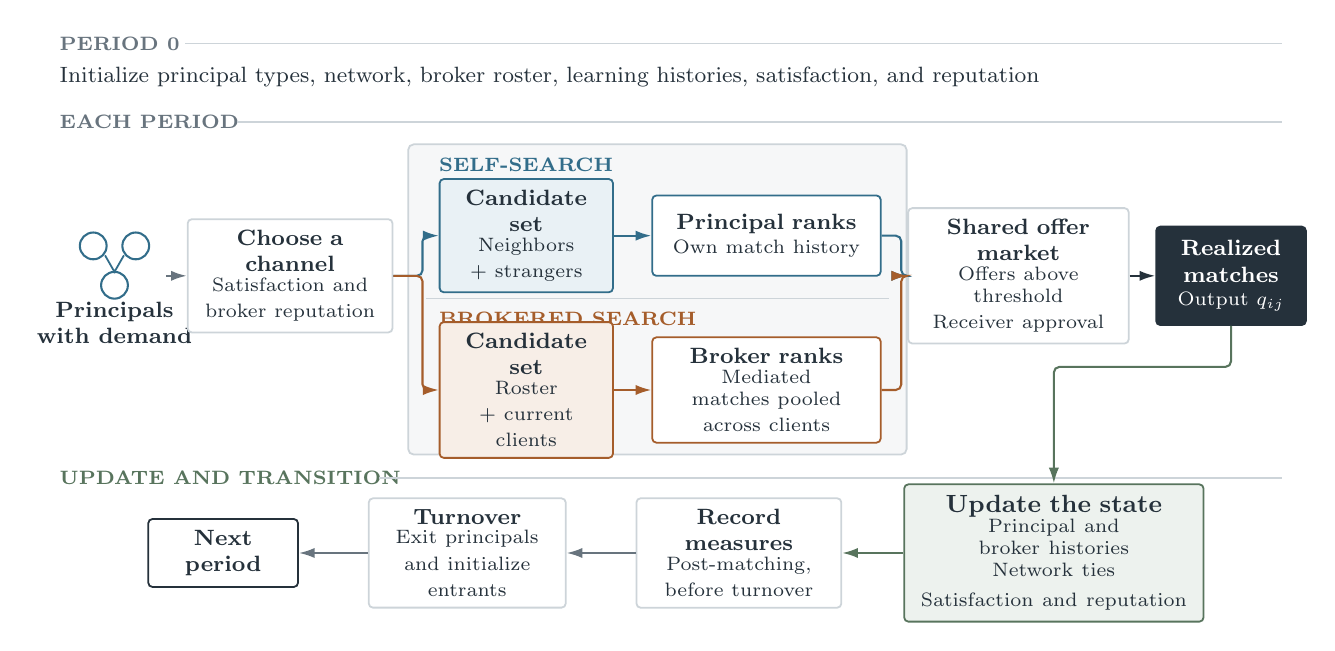
\begin{tikzpicture}[
    x=1cm,
    y=1cm,
    font=\small,
    text=ink,
    >={Latex[length=2.0mm,width=1.3mm]},
    arrow/.style={-{Latex[length=2.0mm,width=1.3mm]}, draw=muted, line width=0.75pt},
    branch/.style={arrow, rounded corners=2pt},
    card/.style={
        draw=rule,
        fill=white,
        rounded corners=1.5pt,
        line width=0.65pt,
        font=\footnotesize,
        align=center,
        inner xsep=5pt,
        inner ysep=4pt
    },
    stage/.style={card, minimum height=1.25cm},
    section/.style={font=\scriptsize\bfseries, text=muted},
    lanehead/.style={font=\scriptsize\bfseries, anchor=west},
    update/.style={
        draw=feedback,
        fill=feedbacklight,
        rounded corners=1.5pt,
        line width=0.65pt,
        align=center,
        inner xsep=5pt,
        inner ysep=4pt
    }
]

% Period-0 setup, presented as context rather than as part of the period loop.
\node[section, anchor=west] at (0,8.10) {PERIOD 0};
\draw[rule, line width=0.6pt] (1.72,8.10) -- (15.65,8.10);
\node[anchor=west, font=\footnotesize] at (0,7.68)
    {Initialize principal types, network, broker roster, learning histories, satisfaction, and reputation};

% Within-period mechanism.
\node[section, anchor=west] at (0,7.10) {EACH PERIOD};
\draw[rule, line width=0.6pt] (2.38,7.10) -- (15.65,7.10);

% Principals and the channel decision.
\begin{scope}[shift={(0.55,5.25)}]
    \draw[self, line width=0.75pt] (0.00,0.28) circle (0.17);
    \draw[self, line width=0.75pt] (0.54,0.28) circle (0.17);
    \draw[self, line width=0.75pt] (0.27,-0.22) circle (0.17);
    \draw[self, line width=0.65pt] (0.15,0.16) -- (0.27,-0.05) -- (0.39,0.16);
\end{scope}
\node[align=center, font=\footnotesize\bfseries] (demand) at (0.82,4.55)
    {Principals\\with demand};

\node[stage, text width=2.25cm] (choice) at (3.05,5.15) {%
    \textbf{Choose a channel}\\[-1pt]
    \scriptsize Satisfaction and\\broker reputation
};
\draw[arrow] (1.48,5.15) -- (choice.west);

% A single comparison panel holds the two search pathways.
\fill[panel, rounded corners=2pt] (4.55,2.88) rectangle (10.88,6.82);
\draw[rule, rounded corners=2pt, line width=0.65pt] (4.55,2.88) rectangle (10.88,6.82);
\draw[rule, line width=0.55pt] (4.78,4.86) -- (10.65,4.86);

\node[lanehead, text=self] at (4.82,6.56) {SELF-SEARCH};
\node[lanehead, text=broker] at (4.82,4.60) {BROKERED SEARCH};

\node[card, draw=self, fill=selflight, text width=1.85cm, minimum height=1.02cm]
    (selfpool) at (6.05,5.66) {%
    \textbf{Candidate set}\\[-1pt]
    \scriptsize Neighbors\\+ strangers
};
\node[card, draw=self, text width=2.55cm, minimum height=1.02cm]
    (selfrank) at (9.10,5.66) {%
    \textbf{Principal ranks}\\[-1pt]
    \scriptsize Own match history
};
\draw[arrow, draw=self] (selfpool.east) -- (selfrank.west);

\node[card, draw=broker, fill=brokerlight, text width=1.85cm, minimum height=1.02cm]
    (brokerpool) at (6.05,3.70) {%
    \textbf{Candidate set}\\[-1pt]
    \scriptsize Roster\\+ current clients
};
\node[card, draw=broker, text width=2.55cm, minimum height=1.02cm]
    (brokerrank) at (9.10,3.70) {%
    \textbf{Broker ranks}\\[-1pt]
    \scriptsize Mediated matches pooled\\across clients
};
\draw[arrow, draw=broker] (brokerpool.east) -- (brokerrank.west);

\draw[branch, draw=self] (choice.east) -- ++(0.37,0) |- (selfpool.west);
\draw[branch, draw=broker] (choice.east) -- ++(0.37,0) |- (brokerpool.west);

% The two channels converge on a common market.
\node[stage, text width=2.45cm] (market) at (12.30,5.15) {%
    \textbf{Shared offer\\market}\\[-1pt]
    \scriptsize Offers above threshold\\Receiver approval
};
\draw[branch, draw=self] (selfrank.east) -- ++(0.25,0) |- (market.west);
\draw[branch, draw=broker] (brokerrank.east) -- ++(0.25,0) |- (market.west);

\node[stage, draw=ink, fill=ink, text=white, text width=1.55cm]
    (matches) at (15.00,5.15) {%
    \textbf{Realized\\matches}\\[-1pt]
    \scriptsize Output $q_{ij}$
};
\draw[arrow, draw=ink] (market.east) -- (matches.west);

% Feedback and transition to the next period.
\node[section, anchor=west, text=feedback] at (0,2.58) {UPDATE AND TRANSITION};
\draw[rule, line width=0.6pt] (4.18,2.58) -- (15.65,2.58);

\node[update, text width=3.45cm] (state) at (12.75,1.63) {%
    \textbf{Update the state}\\[-1pt]
    \scriptsize Principal and broker histories\\Network ties\\Satisfaction and reputation
};
\node[card, text width=2.25cm] (measure) at (8.75,1.63) {%
    \textbf{Record measures}\\[-1pt]
    \scriptsize Post-matching,\\before turnover
};
\node[card, text width=2.15cm] (turnover) at (5.30,1.63) {%
    \textbf{Turnover}\\[-1pt]
    \scriptsize Exit principals\\and initialize entrants
};
\node[card, draw=ink, text width=1.55cm] (next) at (2.20,1.63) {%
    \textbf{Next period}
};

\draw[branch, draw=feedback] (matches.south) -- ++(0,-0.52) -| (state.north);
\draw[arrow, draw=feedback] (state.west) -- (measure.east);
\draw[arrow] (measure.west) -- (turnover.east);
\draw[arrow] (turnover.west) -- (next.east);

\end{tikzpicture}
\end{document}
